\documentclass[conference]{IEEEtran}
\IEEEoverridecommandlockouts
% The preceding line is only needed to identify funding in the first footnote. If that is unneeded, please comment it out.
%Template version as of 6/27/2024

\usepackage{cite}
\usepackage{amsmath,amssymb,amsfonts}
\usepackage{algorithmic}
\usepackage{graphicx}
\usepackage{textcomp}
\usepackage{xcolor}
\usepackage{cite}
\usepackage{enumitem}
\def\BibTeX{{\rm B\kern-.05em{\sc i\kern-.025em b}\kern-.08em
    T\kern-.1667em\lower.7ex\hbox{E}\kern-.125emX}}

% make a new command for umlaut u
\renewcommand{\u}{\"{u}}
\begin{document}

\title{On Genetic Algorithms for the Edge Unfolding of Polytopes}

\author{\IEEEauthorblockN{Dr. Saleha Raza}
\IEEEauthorblockA{\textit{Associate Professor, CS}\\
\textit{Habib University}\\
Karachi, Pakistan \\
saleha.raza@sse.habib.edu.pk}
\and
\IEEEauthorblockN{Musab Kasbati}
\IEEEauthorblockA{\textit{Computer Science}\\
\textit{Habib University}\\
Karachi, Pakistan \\
mk07811@st.habib.edu.pk}
\and  
\IEEEauthorblockN{Raahim Hashmi}
\IEEEauthorblockA{\textit{Computer Science}\\
\textit{Habib University}\\
Karachi, Pakistan \\
rh08461@st.habib.edu.pk}
}

\maketitle

\begin{abstract}
    D\u rer's conjecture states that every polytope has a non-overlapping edge unfolding. It was first proposed in 1975 by Shephard who named it after Albrecht D\u rer, a renowned German artist and mathematician. While there exists algorithms that have been successful at finding non-overlapping edge unfoldings (\emph{nets}) of polytopes, there exists no proof of their correctness. As the possible unfoldings is exponential in the features of the polytope, such as its number of faces or number of vertices, we found that it was worth investigating a meta-heuristic approach that explores the vast search space and outputs an unfolding with minimal, and ideally zero, overlaps. 
\end{abstract}

\begin{IEEEkeywords}
polytopes, unfolding, computational geometry, genetic algorithms, d\u rer's conjecture
\end{IEEEkeywords}

\section{Introduction}
The term polytope can be ambiguous due to different meanings across literature. For this report, we define polytopes as three-dimensional bounded convex polyhedrons. An unfolding, or specifically, an edge-unfolding of a polytope can be thought of as cutting the polytope along its edges and laying its faces out flat in a two-dimensional plane such that no faces are disconnected (see Figure \ref{fig:example1}). A \emph{net} is an edge-unfolding of a polytope such that the faces do not overlap. Whether or not every polytope has a net is an open problem in computational geometry known as D\u rer's Conjecture, first proposed by Shephard in 1975 and named after Albrecht D\u rer, a renowned German artist and mathematician whose book ``Underweysung der Messung'' (Instruction in Measurement with Compass and Straightedge) contributed greatly to the understanding of polyhedra and their two-dimensional unfoldings.

\begin{figure}[!h]
    \centering
    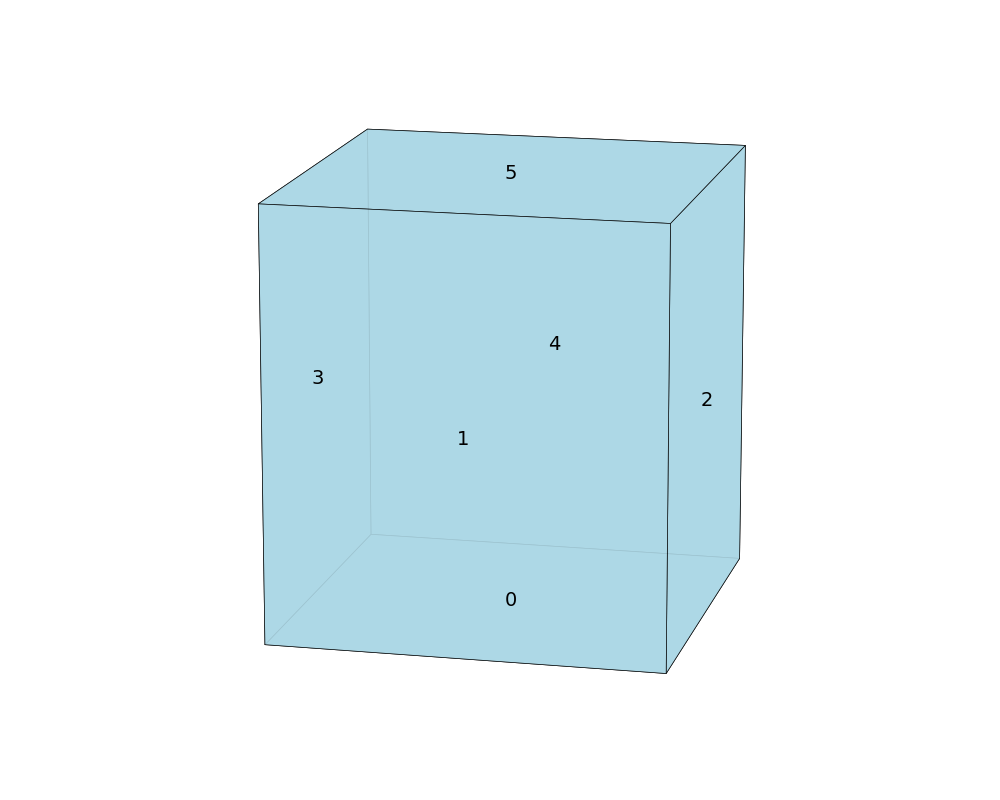
\includegraphics[width=0.2\textwidth]{figures/ex1cube.png}
    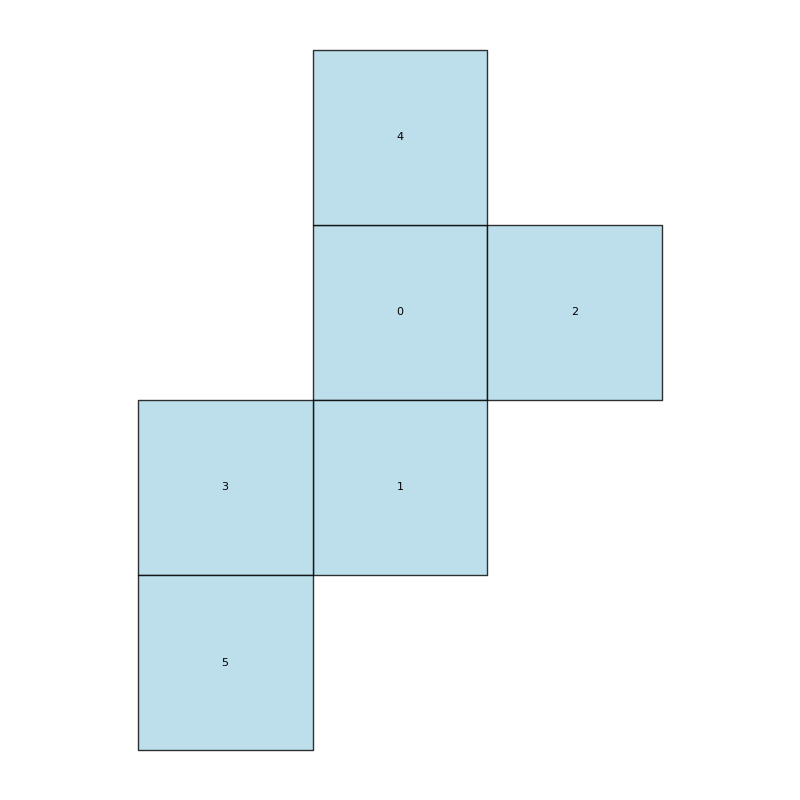
\includegraphics[width=0.2\textwidth]{figures/ex1cubeunfolding2.png} 
    \caption{An example of a cube and one of its possible nets.}
    \label{fig:example1}
\end{figure}

The natural approach of cutting along the edges to obtain an unfolding of a polytope can be formally defined as obtaining a \emph{cut-graph} $G_c = (V_c, E_c)$ such that $G_c$ is a spanning tree of the polytope's vertex graph $G_p = (V, E)$ where $V$ is the set of vertices of the polytope and $E$ is the set of edges between the vertices. The edge set $E_c$ are the edges to cut along to obtain an unfolding. It can be proven that cutting the edges in any spanning tree of $G_p$ gives an unfolding for the polytope (Lemma 22.1.1 of \cite{demaineGeometricFoldingAlgorithms2007}). It can also be proven that for every cut-graph $G_c$, there exists a \emph{join-graph} $G_j = (V_j, E_j)$ that is a spanning tree of the polytope's face/dual graph $G_f = (V_f, E_f)$, where $V_f$ is the set of faces of the polytope and $(u, v) \in E_f$ if $u, v \in V_f$ and there exists a common edge between the faces $u$ and $v$ (Lemma 2.2 of \cite{schlickenriederNetsPolyhedra}). While a cut-graph presents a natural way of obtaining an unfolding, that is by cutting along its edges, the join-graph turns out to be computationally easier to deal with and is a simpler way to view the unfolding, e.g. the unfolding in figure \ref{fig:example1} can be viewed as a join-tree of the dual graph of the cube. 

It is important to note that not all spanning trees result in unfoldings that are nets, and as such, the problem of finding nets of a polytope reduces to finding a cut-graph or a join-graph that results in a net. As the number of spanning trees for a given graph can be exponential in the number of vertices, it is not possible to check all spanning trees to find a net. Work has been done on designing algorithms that attempt to produce a net for a given polytope by generating a spanning tree according to some heuristic; however, no algorithm has been proven to always find a net, despite algorithms existing that have always succeeded to find a net for given polytopes. In this report, we present, to the best of our knowledge, the first metaheuristic approach for finding nets of polytopes. We use a genetic algorithm to obtain a spanning tree of the polytope's dual graph and compare the results with existing algorithms. 

\section{Related Work}

The most substantial resource on algorithms for finding nets of polytopes is the thesis of Schlickenrieder \cite{schlickenriederNetsPolyhedra}. In his thesis, Schlickenrieder explores 24 algorithms that take in a vertex-graph or a face-graph of a polytope and output a spanning tree. The algorithms include common graph algorithms such as \textsc{Breadth-First-Search} and \textsc{Depth-First-Search}, algorithms to test his or other's conjectures such as \textsc{Min-Perimeter} which produces a minimum spanning tree of the vertex graph to to test a conjecture that the unfolding with minimal perimeter is always a net, as well as algorithms that are combine aspects or heuristics of other algorithms. He tested the algorithms on a dataset of about 10000 polytopes and measured the percentage of produced unfoldings that had overlaps as the metric of the algorithm's performance. Among the algorithms he tested, the \textsc{Steepest-Edge-Unfold} algorithm was the most successful, with only 1.2\% of produced unfoldings having overlaps. The algorithm is based on his conjecture that cutting along the edges that are the ``straightest'' according to some metric can produce a net. For this purpose, the algorithm works by randomly generating a unit vector and taking the vertex that is least in the direction of the vector as the root. Then, from each vertex, it selects edges that are the most in the direction of the vector. Due to the random nature of the algorithm, running it multiple times can produce different unfoldings. Schlickenrieder found that \textsc{Steepest-Edge-Unfold} always managed to produce a net within 7 attempts for all the polytopes in his dataset.  

\section{Methodology}

\subsection{Genetic Algorithms}

Genetic algorithms (GAs) are a class of metaheuristic optimization algorithms used for combinatorial problems. They are fundamentally inspired by biological evolution and natural selection. GAs work by maintaining a generation of \emph{candidates} which are possible solutions to the problem, iteratively improving upon them through operations that mimic biological processes such as genetic recombination and mutation, and selecting the fittest candidates to survive to the next generation. A GA is typically composed of the following steps:

\begin{enumerate}[label=(\arabic*)]
    \item \textbf{Initialization:} A population of candidates is randomly generated.
    \item \textbf{Evaluation:} Each candidate is evaluated using a fitness function that measures how well it solves the problem.
    \item \textbf{Parent Selection:} Candidates are selected to be parents based on some selection scheme, such as rank-based selection or binary tournament selection.
    \item \textbf{Crossover:} The information of parent solutions is combined to create offspring candidates. A \emph{crossover operator}, such as uniform crossover or two-point crossover, is used for this purpose.
    \item \textbf{Mutation:} Based on some small probability, the offsprings undergo a small mutation that alters their information, potentially introducing new information to the population. A \emph{mutation operator} is used for this purpose.
    \item \textbf{Survivor Selection:} The next generation of candidates is selected from the current generation and the offspring based on some selection scheme, such as truncation or fitness-proportionate selection.
    \item \textbf{Termination:} Steps 2-6 are repeated until a termination condition is met, such as a maximum number of generations or the population converging to a solution.
\end{enumerate}

To facilitate this proceedure, a representation of the candidate solution, called a \emph{chromosome}, a fitness function, and crossover and mutation operators are required. The size of the population, parent and survivor selection schemes, and the mutation probability are also typical hyperparameters of a GA that can be tuned to improve the its performance.

\subsection{GA for Unfolding Polytopes}

Our GA for unfolding polytopes takes in a polytope's dual graph and maintains a population of candidate solutions that can be converted to join-graphs. It aims to minimize the number of overlaps in the produced unfoldings.

\subsubsection{Chromosome Representation}

For each candidate, we maintained an array of length $|E_f|$ of integers between 0 and $|E_f| - 1$ such that the $i$-th index represented the weight of the $i$-th edge in the dual graph. To convert the chromosome to a join-graph, we simply used Prim's Algorithm to obtain the minimum spanning tree of the dual graph with the weights of the edges set to the values in the chromosome. This representation allowed us to easily initialized a random population of candidates, as well as apply crossover and mutation operators with little consideration regarding the validity of the resulting candidates.

\subsubsection{Fitness Function}
The fitness of a candidate was taken to be the number of overlaps in the unfolding produced by the join-graph of the candidate. To check for the number of overlaps, we relied on the Separating Axis Theorem (SAT) which states that two convex shapes do not overlap if and only if there exists an axis such that the projections of the two shapes on the axis do not overlap. Additionally, we can significantly reduce the number of axes we need to check by only checking the axes formed by the normal vectors of the faces of the polytope. Furthermore, instead of comparing every pair of faces, we can do what is called a \emph{broad-phase check} by first comparing the $x$ coordinates of the bounding boxes of the faces. If the bounding boxes do not overlap, we can skip checking the pair of faces as they cannot possibly overlap. Once we have the pair of faces for whom we do need to check for overlap, we can use the SAT for a \emph{narrow-phase check}. Once we have the number of overlaps, we can simply use that as a fitness value for the candidate.

\subsubsection{Crossover and Mutation Operators}

We used a uniform crossover operator which builds the offsprings by tossing a coin for each index in the parents' chromosomes and taking the value from one of the parents. This was mostly unproblematic; however, it did leave room for multiple edges to have the same weight which isn't an issue immediately but may have caused issues if allowed to persist. To deal with this, we permuted the edges that had the same weights so that their order with respect to each other was not preserved because - ?

\subsection{Generating Polytopes}

In order to generate polytopes for testing our GA, we identified a few categories of polytopes from Schlickenrieder's thesis \cite{schlickenriederNetsPolyhedra} that were among the hardest to unfold. The categories we used were:
\begin{itemize}
    \item \textbf{Uniform Polytopes:} These are polytopes that were generated by taking the convex hull of $n$ points in the bounding box defined by the vertices in $\{-n, n\} \times \{-n, n\} \times \{-n, n\}$. 
    \item \textbf{Flat Polytopes:} The generation of these polytopes was similar to the uniform polytopes, except that with a 0.7 probability, the $i$-th point would have the same $x$ and $y$ coordinates as the $(i-1)$-th point with its $z$ coordinate equal to $-n$ where $n$ is the total number of points. Note that the first point was generated randomly in the same bounding box as the uniform polytopes. This generation gives a polytope with a higher number of faces that have more than 3 vertices.
    \item \textbf{Spherical Polytopes:} These polytopes were generated by taking the convex hull of $n$ points on the surface of a unit sphere. The points were generated by taking random values of $\theta$ in the range $[0, 2\pi]$ and $\phi$ in the range $[0, \pi]$ respectively and inputting them into the parametrized equation of the sphere: $\langle \sin(\phi)\cos(\theta), \sin(\phi)\sin(\theta), \cos(\phi) \rangle$.
    \item \textbf{Half-spherical Polytopes:} These polytopes were generated in the same way as the spherical polytopes, with the range of $\phi$ being $[0, \pi/2]$ instead of $[0, \pi]$. The resultant polytope has a relatively flat base and points concentrated to the top of the polytope.
    \item \textbf{Turtle Polytopes:} The vertices for these polytopes were points in the set $\{(x, y, x^2 + y^2) \mid x \in \{-i, -i + 1, \ldots, i\}, y \in \{-j, -j + 1, \ldots, j\}\}$ where $i$ and $j$ were randomly chosen integers in the range $[1, 7]$. 
\end{itemize}

\subsection{Visualization}

Once the points of the polytopes were generated, we obtained their convex hull and the simplices (triangulations of faces) of the resulting polytope using functions from Python's \texttt{scipy} library. Then, we merged those simplices by obtaining their plane equations and taking the union of the points of the simplices that had the same plane equation. This allowed us to obtain the faces of the resulting polytopes. Furthermore, we sorted the points with respect to their angle with the centroid of the face in order to figure out the edges between the points of the face; with this ordering, there was an edge between two consecutive points and the first and last point. To obtain the dual graph of the polytope, we initialized a graph with the faces of the polytope as its nodes and an empty edge set. We then iterated through the faces and added an edge between two faces if they had an edge in common.

After obtaining the dual graph, we could proceed with obtaining unfoldings of the polytope. However, we still needed to visualize the unfolding. For this, we first fixed the orientation of the vertices in the array defining a face. As two adjacent faces must share an edge, that is they have two vertices in common and in both faces they appear consecutively, we made sure that the two vertices were in the same order in both faces. This required simply reversing the order of the vertices in one of the faces if they were not in the same order as the other face. 

\subsection{Abbreviations and Acronyms}
% Define abbreviations and acronyms the first time they are used in the text, 
% even after they have been defined in the abstract. Abbreviations such as 
% IEEE, SI, MKS, CGS, ac, dc, and rms do not have to be defined. Do not use 
% abbreviations in the title or heads unless they are unavoidable.

\subsection{Units}
% \begin{itemize}
% \item Use either SI (MKS) or CGS as primary units. (SI units are encouraged.) English units may be used as secondary units (in parentheses). An exception would be the use of English units as identifiers in trade, such as ``3.5-inch disk drive''.
% \item Avoid combining SI and CGS units, such as current in amperes and magnetic field in oersteds. This often leads to confusion because equations do not balance dimensionally. If you must use mixed units, clearly state the units for each quantity that you use in an equation.
% \item Do not mix complete spellings and abbreviations of units: ``Wb/m\textsuperscript{2}'' or ``webers per square meter'', not ``webers/m\textsuperscript{2}''. Spell out units when they appear in text: ``. . . a few henries'', not ``. . . a few H''.
% \item Use a zero before decimal points: ``0.25'', not ``.25''. Use ``cm\textsuperscript{3}'', not ``cc''.)
% \end{itemize}

\subsection{Equations}
% Number equations consecutively. To make your 
% equations more compact, you may use the solidus (~/~), the exp function, or 
% appropriate exponents. Italicize Roman symbols for quantities and variables, 
% but not Greek symbols. Use a long dash rather than a hyphen for a minus 
% sign. Punctuate equations with commas or periods when they are part of a 
% sentence, as in:
% \begin{equation}
% a+b=\gamma\label{eq}
% \end{equation}

% Be sure that the 
% symbols in your equation have been defined before or immediately following 
% the equation. Use ``\eqref{eq}'', not ``Eq.~\eqref{eq}'' or ``equation \eqref{eq}'', except at 
% the beginning of a sentence: ``Equation \eqref{eq} is . . .''

\subsection{\LaTeX-Specific Advice}

% Please use ``soft'' (e.g., \verb|\eqref{Eq}|) cross references instead
% of ``hard'' references (e.g., \verb|(1)|). That will make it possible
% to combine sections, add equations, or change the order of figures or
% citations without having to go through the file line by line.

% Please don't use the \verb|{eqnarray}| equation environment. Use
% \verb|{align}| or \verb|{IEEEeqnarray}| instead. The \verb|{eqnarray}|
% environment leaves unsightly spaces around relation symbols.

% Please note that the \verb|{subequations}| environment in {\LaTeX}
% will increment the main equation counter even when there are no
% equation numbers displayed. If you forget that, you might write an
% article in which the equation numbers skip from (17) to (20), causing
% the copy editors to wonder if you've discovered a new method of
% counting.

% {\BibTeX} does not work by magic. It doesn't get the bibliographic
% data from thin air but from .bib files. If you use {\BibTeX} to produce a
% bibliography you must send the .bib files. 

% {\LaTeX} can't read your mind. If you assign the same label to a
% subsubsection and a table, you might find that Table I has been cross
% referenced as Table IV-B3. 

% {\LaTeX} does not have precognitive abilities. If you put a
% \verb|\label| command before the command that updates the counter it's
% supposed to be using, the label will pick up the last counter to be
% cross referenced instead. In particular, a \verb|\label| command
% should not go before the caption of a figure or a table.

% Do not use \verb|\nonumber| inside the \verb|{array}| environment. It
% will not stop equation numbers inside \verb|{array}| (there won't be
% any anyway) and it might stop a wanted equation number in the
% surrounding equation.

\subsection{Some Common Mistakes}
% \begin{itemize}
% \item The word ``data'' is plural, not singular.
% \item The subscript for the permeability of vacuum $\mu_{0}$, and other common scientific constants, is zero with subscript formatting, not a lowercase letter ``o''.
% \item In American English, commas, semicolons, periods, question and exclamation marks are located within quotation marks only when a complete thought or name is cited, such as a title or full quotation. When quotation marks are used, instead of a bold or italic typeface, to highlight a word or phrase, punctuation should appear outside of the quotation marks. A parenthetical phrase or statement at the end of a sentence is punctuated outside of the closing parenthesis (like this). (A parenthetical sentence is punctuated within the parentheses.)
% \item A graph within a graph is an ``inset'', not an ``insert''. The word alternatively is preferred to the word ``alternately'' (unless you really mean something that alternates).
% \item Do not use the word ``essentially'' to mean ``approximately'' or ``effectively''.
% \item In your paper title, if the words ``that uses'' can accurately replace the word ``using'', capitalize the ``u''; if not, keep using lower-cased.
% \item Be aware of the different meanings of the homophones ``affect'' and ``effect'', ``complement'' and ``compliment'', ``discreet'' and ``discrete'', ``principal'' and ``principle''.
% \item Do not confuse ``imply'' and ``infer''.
% \item The prefix ``non'' is not a word; it should be joined to the word it modifies, usually without a hyphen.
% \item There is no period after the ``et'' in the Latin abbreviation ``et al.''.
% \item The abbreviation ``i.e.'' means ``that is'', and the abbreviation ``e.g.'' means ``for example''.
% \end{itemize}
% An excellent style manual for science writers is \cite{b7}.

\subsection{Authors and Affiliations}
% \textbf{The class file is designed for, but not limited to, six authors.} A 
% minimum of one author is required for all conference articles. Author names 
% should be listed starting from left to right and then moving down to the 
% next line. This is the author sequence that will be used in future citations 
% and by indexing services. Names should not be listed in columns nor group by 
% affiliation. Please keep your affiliations as succinct as possible (for 
% example, do not differentiate among departments of the same organization).

% \subsection{Identify the Headings}\label{ITH}
% Headings, or heads, are organizational devices that guide the reader through 
% your paper. There are two types: component heads and text heads.

% Component heads identify the different components of your paper and are not 
% topically subordinate to each other. Examples include Acknowledgments and 
% References and, for these, the correct style to use is ``Heading 5''. Use 
% ``figure caption'' for your Figure captions, and ``table head'' for your 
% table title. Run-in heads, such as ``Abstract'', will require you to apply a 
% style (in this case, italic) in addition to the style provided by the drop 
% down menu to differentiate the head from the text.

% Text heads organize the topics on a relational, hierarchical basis. For 
% example, the paper title is the primary text head because all subsequent 
% material relates and elaborates on this one topic. If there are two or more 
% sub-topics, the next level head (uppercase Roman numerals) should be used 
% and, conversely, if there are not at least two sub-topics, then no subheads 
% should be introduced.

% \subsection{Figures and Tables}\label{FAT}
% \paragraph{Positioning Figures and Tables} Place figures and tables at the top and 
% bottom of columns. Avoid placing them in the middle of columns. Large 
% figures and tables may span across both columns. Figure captions should be 
% below the figures; table heads should appear above the tables. Insert 
% figures and tables after they are cited in the text. Use the abbreviation 
% ``Fig.~\ref{fig}'', even at the beginning of a sentence.

% \begin{table}[htbp]
% \caption{Table Type Styles}
% \begin{center}
% \begin{tabular}{|c|c|c|c|}
% \hline
% \textbf{Table}&\multicolumn{3}{|c|}{\textbf{Table Column Head}} \\
% \cline{2-4} 
% \textbf{Head} & \textbf{\textit{Table column subhead}}& \textbf{\textit{Subhead}}& \textbf{\textit{Subhead}} \\
% \hline
% copy& More table copy$^{\mathrm{a}}$& &  \\
% \hline
% \multicolumn{4}{l}{$^{\mathrm{a}}$Sample of a Table footnote.}
% \end{tabular}
% \label{tab1}
% \end{center}
% \end{table}

% \begin{figure}[htbp]
% \centerline{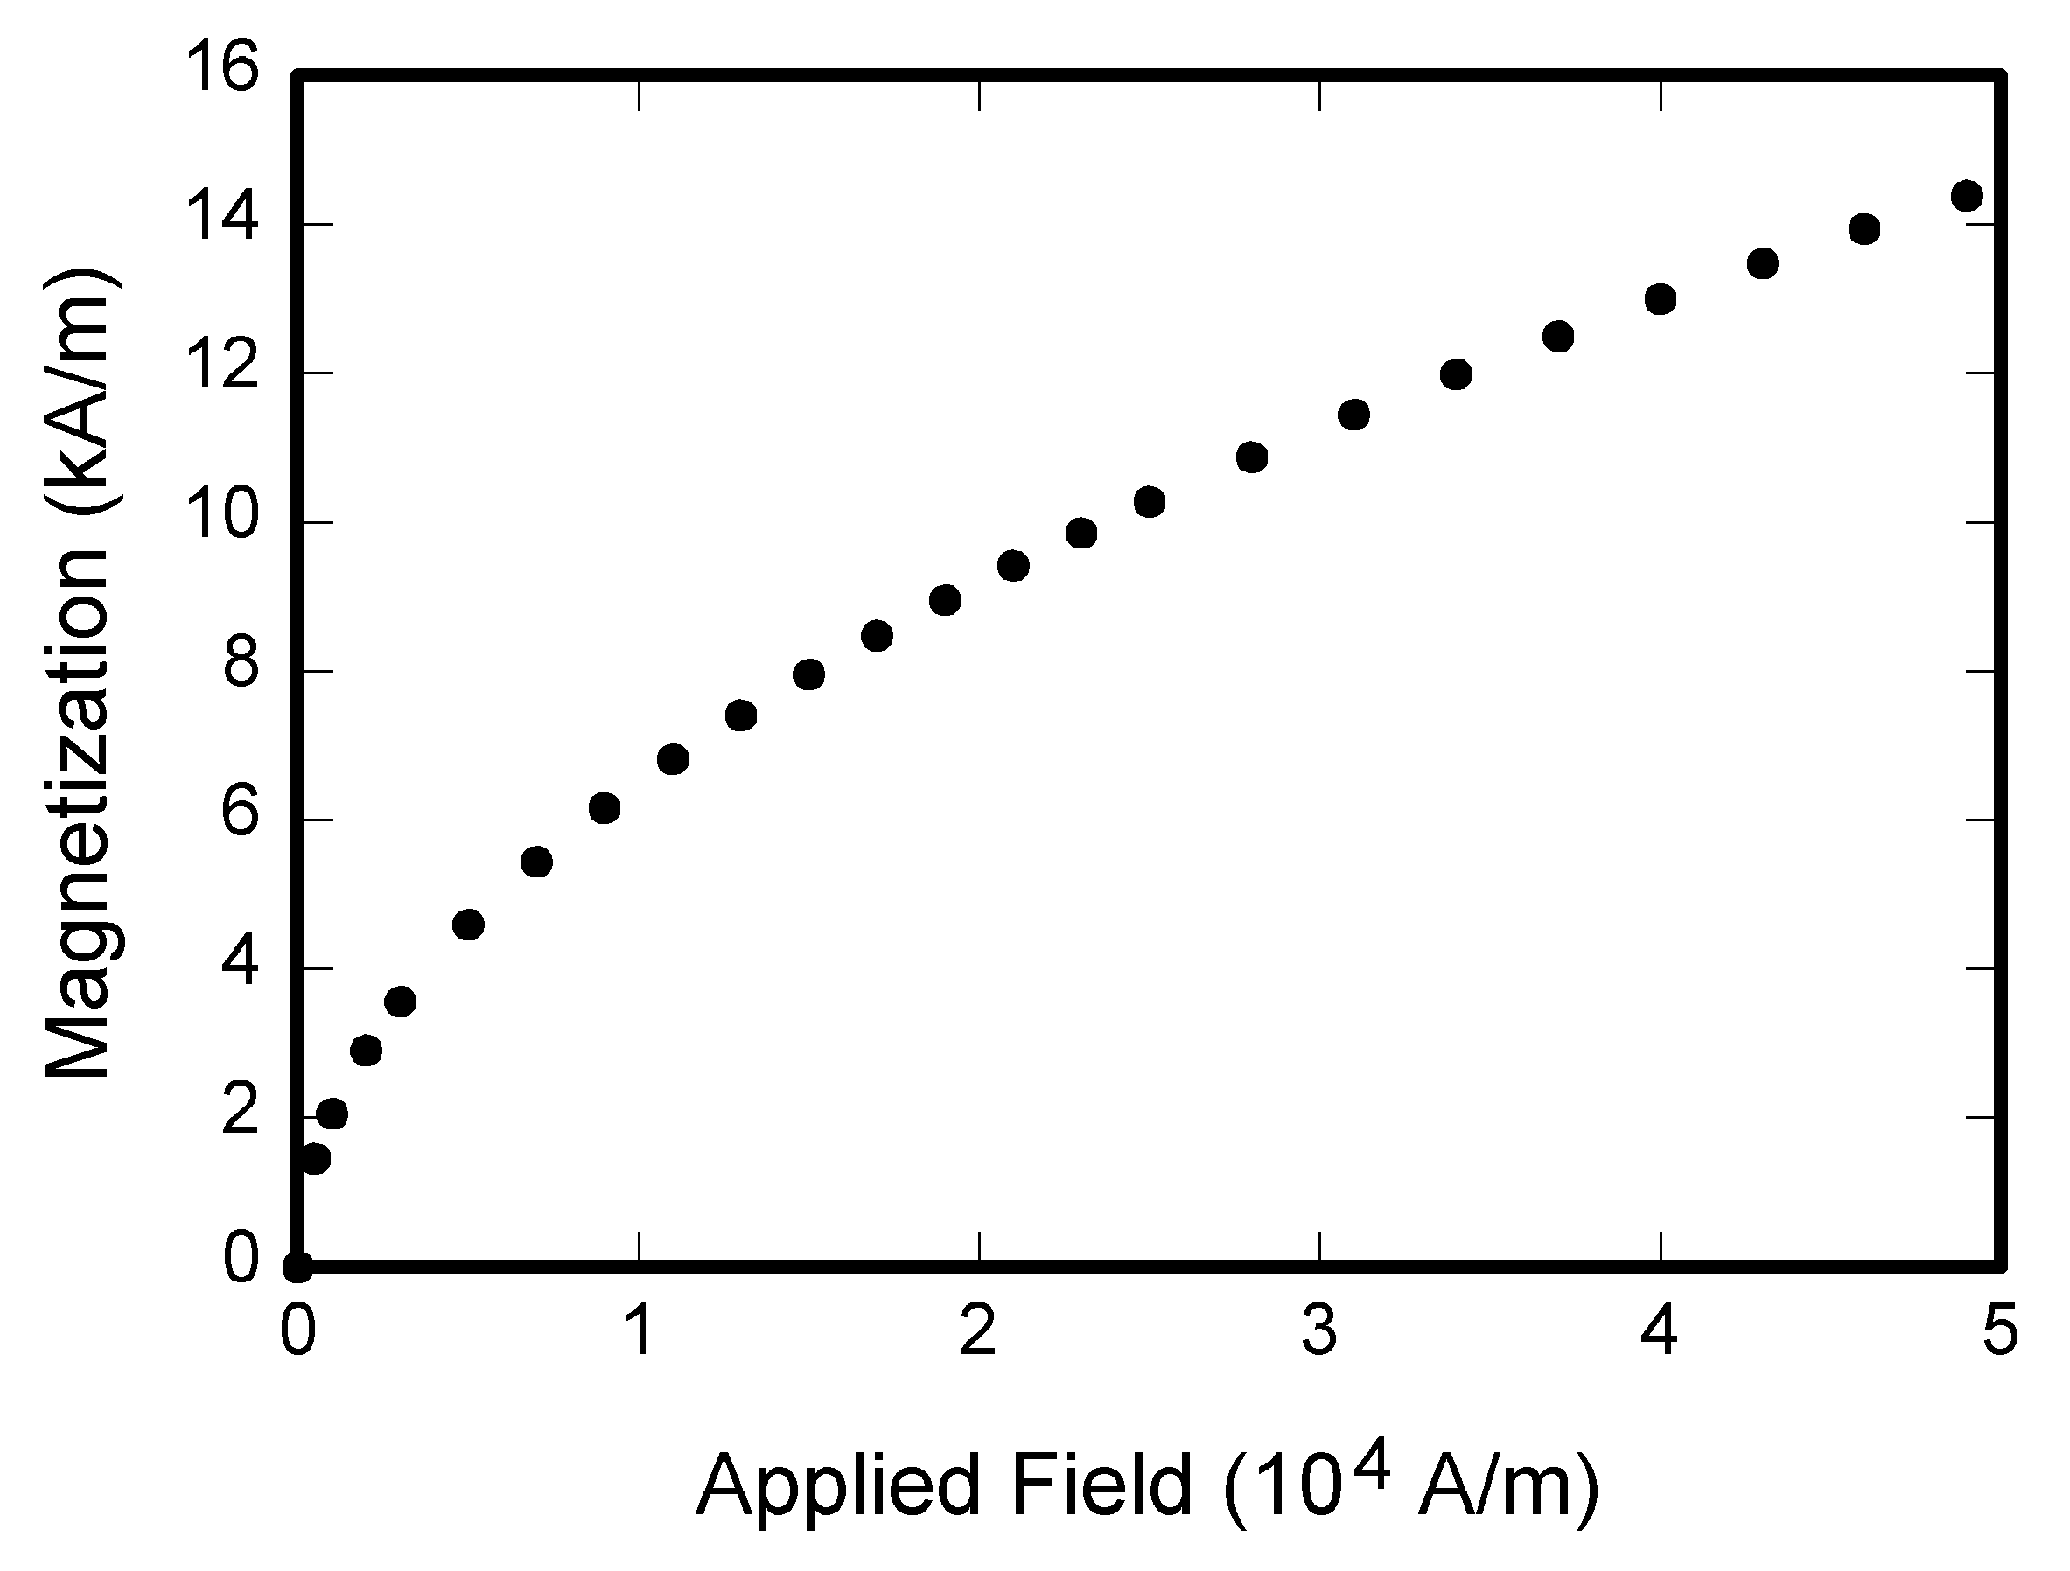
\includegraphics{fig1.png}}
% \caption{Example of a figure caption.}
% \label{fig}
% \end{figure}

% Figure Labels: Use 8 point Times New Roman for Figure labels. Use words 
% rather than symbols or abbreviations when writing Figure axis labels to 
% avoid confusing the reader. As an example, write the quantity 
% ``Magnetization'', or ``Magnetization, M'', not just ``M''. If including 
% units in the label, present them within parentheses. Do not label axes only 
% with units. In the example, write ``Magnetization (A/m)'' or ``Magnetization 
% \{A[m(1)]\}'', not just ``A/m''. Do not label axes with a ratio of 
% quantities and units. For example, write ``Temperature (K)'', not 
% ``Temperature/K''.

\section*{Acknowledgment}

% The preferred spelling of the word ``acknowledgment'' in America is without 
% an ``e'' after the ``g''. Avoid the stilted expression ``one of us (R. B. 
% G.) thanks $\ldots$''. Instead, try ``R. B. G. thanks$\ldots$''. Put sponsor 
% acknowledgments in the unnumbered footnote on the first page.

\section*{References}

% Please number citations consecutively within brackets \cite{b1}. The 
% sentence punctuation follows the bracket \cite{b2}. Refer simply to the reference 
% number, as in \cite{b3}---do not use ``Ref. \cite{b3}'' or ``reference \cite{b3}'' except at 
% the beginning of a sentence: ``Reference \cite{b3} was the first $\ldots$''

% Number footnotes separately in superscripts. Place the actual footnote at 
% the bottom of the column in which it was cited. Do not put footnotes in the 
% abstract or reference list. Use letters for table footnotes.

% Unless there are six authors or more give all authors' names; do not use 
% ``et al.''. Papers that have not been published, even if they have been 
% submitted for publication, should be cited as ``unpublished'' \cite{b4}. Papers 
% that have been accepted for publication should be cited as ``in press'' \cite{b5}. 
% Capitalize only the first word in a paper title, except for proper nouns and 
% element symbols.

% For papers published in translation journals, please give the English 
% citation first, followed by the original foreign-language citation \cite{b6}.

\bibliographystyle{IEEEtran}
\bibliography{Unfolding.bib}

% \begin{thebibliography}{00}
% \bibitem{b1} G. Eason, B. Noble, and I. N. Sneddon, ``On certain integrals of Lipschitz-Hankel type involving products of Bessel functions,'' Phil. Trans. Roy. Soc. London, vol. A247, pp. 529--551, April 1955.
% \bibitem{b2} J. Clerk Maxwell, A Treatise on Electricity and Magnetism, 3rd ed., vol. 2. Oxford: Clarendon, 1892, pp.68--73.
% \bibitem{b3} I. S. Jacobs and C. P. Bean, ``Fine particles, thin films and exchange anisotropy,'' in Magnetism, vol. III, G. T. Rado and H. Suhl, Eds. New York: Academic, 1963, pp. 271--350.
% \bibitem{b4} K. Elissa, ``Title of paper if known,'' unpublished.
% \bibitem{b5} R. Nicole, ``Title of paper with only first word capitalized,'' J. Name Stand. Abbrev., in press.
% \bibitem{b6} Y. Yorozu, M. Hirano, K. Oka, and Y. Tagawa, ``Electron spectroscopy studies on magneto-optical media and plastic substrate interface,'' IEEE Transl. J. Magn. Japan, vol. 2, pp. 740--741, August 1987 [Digests 9th Annual Conf. Magnetics Japan, p. 301, 1982].
% \bibitem{b7} M. Young, The Technical Writer's Handbook. Mill Valley, CA: University Science, 1989.
% \bibitem{b8} D. P. Kingma and M. Welling, ``Auto-encoding variational Bayes,'' 2013, arXiv:1312.6114. [Online]. Available: https://arxiv.org/abs/1312.6114
% \bibitem{b9} S. Liu, ``Wi-Fi Energy Detection Testbed (12MTC),'' 2023, gitHub repository. [Online]. Available: https://github.com/liustone99/Wi-Fi-Energy-Detection-Testbed-12MTC
% \bibitem{b10} ``Treatment episode data set: discharges (TEDS-D): concatenated, 2006 to 2009.'' U.S. Department of Health and Human Services, Substance Abuse and Mental Health Services Administration, Office of Applied Studies, August, 2013, DOI:10.3886/ICPSR30122.v2
% \bibitem{b11} K. Eves and J. Valasek, ``Adaptive control for singularly perturbed systems examples,'' Code Ocean, Aug. 2023. [Online]. Available: https://codeocean.com/capsule/4989235/tree
% \end{thebibliography}

% \vspace{12pt}
% \color{red}
% IEEE conference templates contain guidance text for composing and formatting conference papers. Please ensure that all template text is removed from your conference paper prior to submission to the conference. Failure to remove the template text from your paper may result in your paper not being published.

\end{document}
